%\begin{figure}[h]
	%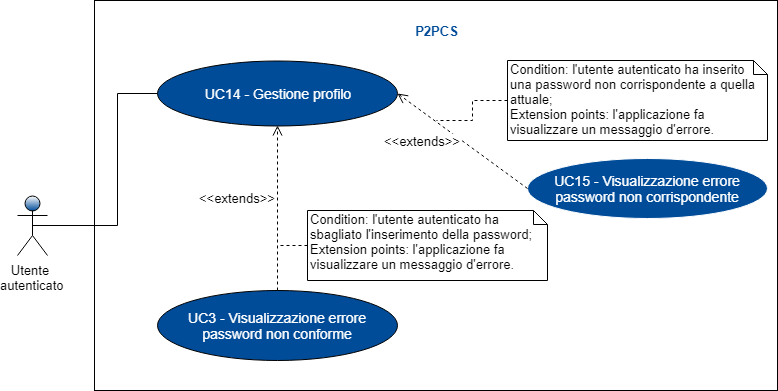
\includegraphics[width=15cm]{res/images/Schemagenerale5.png}
	%\centering
	%\caption{Schema generale: gestione profilo ed errori annessi}
%\end{figure}

Una volta che i giocatori salgono di livello (il loro "traguardo temporale"), vogliono naturalmente vedere quali sono queste nuove abilità, metterle alla prova un po ', metterle alla prova su nemici più forti, godere di quanto sono potenti e poi rendersi conto di essere così vicine alla prossima pietra miliare che potrebbero anche arrivare prima.


\subsubsection{UC20 - Milestone Unlock}
\begin{itemize}
	\item \textbf{Attori Primari}: utente autenticato;
	\item \textbf{Descrizione}: l'applicazione fornisce una tabella Milestone Unlock\glosp che illustra quali premi verranno sbloccati quando si raggiungono certi livelli esperienza. Quando l'utente raggiunge un nuovo livello di esperienza presente nella tabella, sblocca il corripendente premio;	
	\item \textbf{Scenario principale}: l'utente ha raggiunto un nuovo livello di esperinza, presente nella tabella Milestone Unlock. 
	I premi possono essere del seguente tipo:
	\begin{itemize}
		\item aumento del valore del prossimo buono sconto che si andrà a ricevere (x\% in piu');
		\item sconto dell'x\% sul prossimo acquisto nel negozio dell'app;
		\item beni virtuali.
	\end{itemize}
	\item \textbf{Precondizione}: l'utente è in possesso di un account all'interno del sistema. Deve quindi essersi registrato e non aver eliminato l'account;
	\item \textbf{Postcondizione}: l'utente ha effettuato l'operazione di modifica dati oppure l'eliminazione dell'account e il processo è stato confermato dal sistema.
	\item \textbf{Estensioni}:
	\begin{itemize}
		\item visualizzazione errore email non valida [UC2];
		\item visualizzazione errore password non conforme [UC3];
		\item visualizzazione errore password non corrispondente [UC15].
	\end{itemize}
\end{itemize}
\begin{figure}[h]
	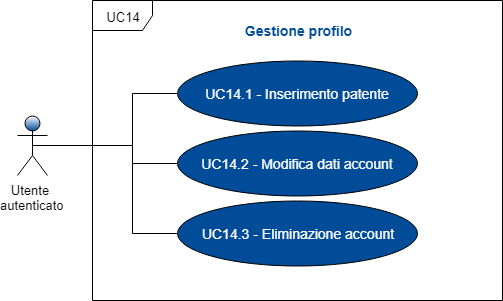
\includegraphics[width=10cm]{res/images/UC14Profilo.png}
	\centering
	\caption{UC14 - Gestione Profilo}
\end{figure} 


